\documentclass{article}
\usepackage{amsmath}
\usepackage{graphicx} % Required for inserting images
\usepackage[utf8]{inputenc}

\title{MRM reliability}
\author{Ashwyn Srinivasan}
\date{July 2024}

\begin{document}

%\maketitle

Black's equation to calculate the heater reliability with current density and ambient temperature ($\rm{T_{ambient}}$):
\begin{equation}
MTTF(J,T_{ambient}) = \frac{A_{MTTF}}{J^{n}} \cdot exp(\frac{E_A}{k_B T_{ambient}})
\end{equation}
To convert  Black's equation from ambient temperature to local heater temperature ($\rm{T_{joule}}$), we need:
\begin{equation}
MTTF(T_{joule}) = A_{MTTF} \cdot exp(\frac{E_A}{k_B T_{joule}})
\end{equation}
Next step is to determine the failure-rate and activation energy from the following 2 figures
\begin{figure}[htp]
	\centering
	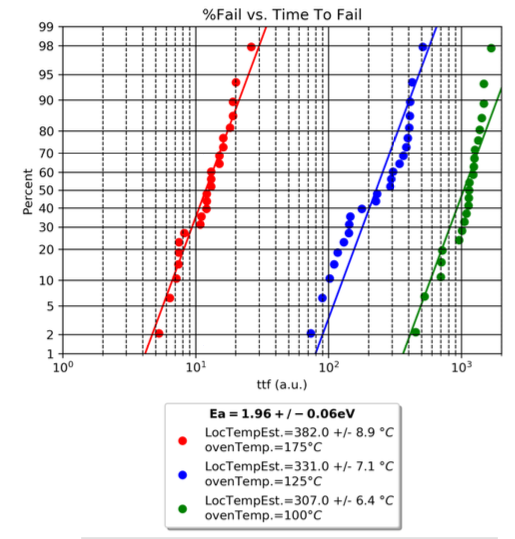
\includegraphics[width=8cm]{figure_5.png}
	\caption{Cumulative distribution of failure vs. time to failure at three oven temperatures. Both the oven temperature and the estimated local heater temperature are shown. }
	\label{fig:gffig5}
\end{figure}
\begin{figure}[htp]
	\centering
	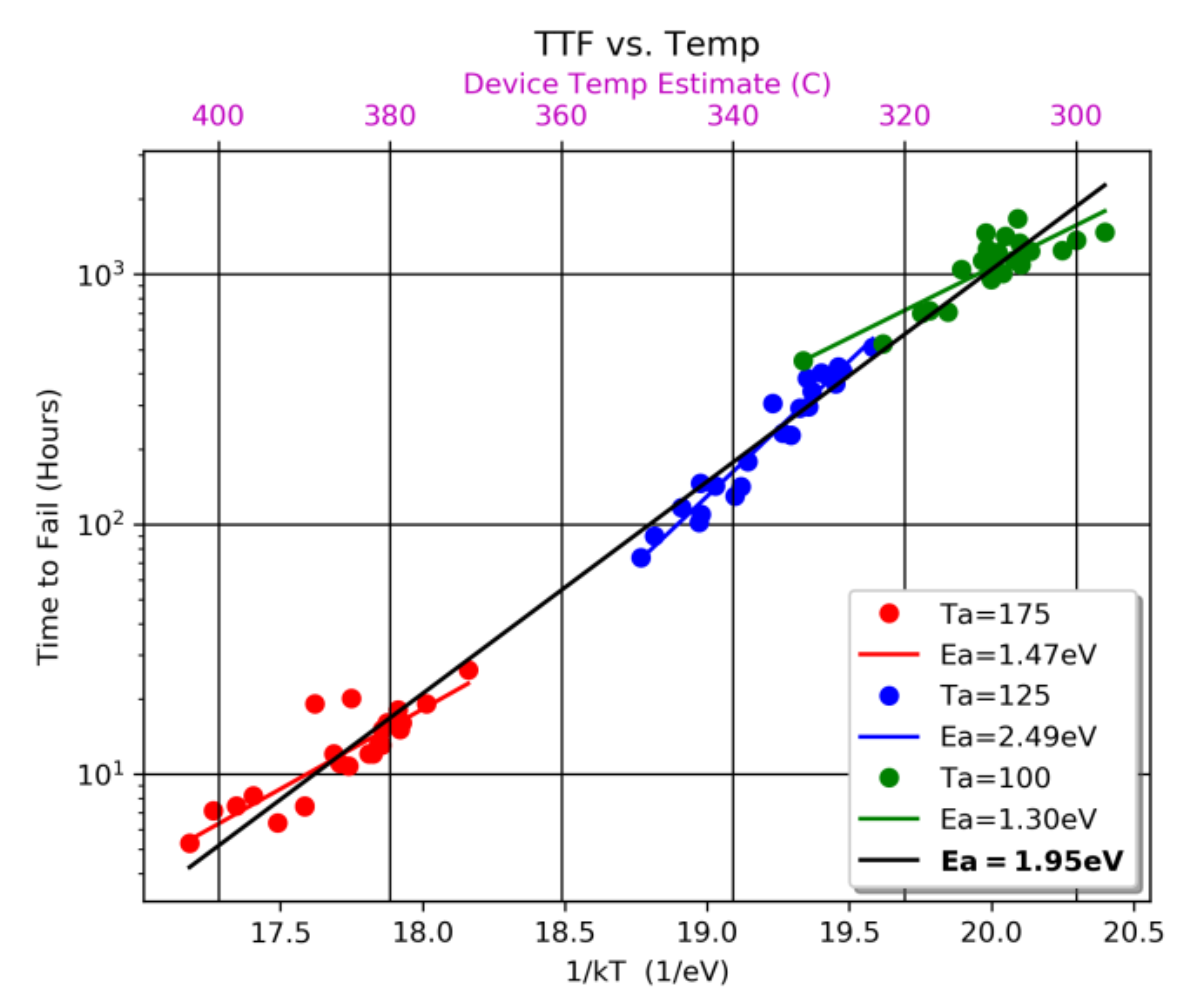
\includegraphics[width=8cm]{figure_6.png}
	\caption{Time to failure vs local temperature for each individual device. Devices were stressed at three different oven temperatures.}
	\label{fig:gffig6}
\end{figure}
\section{Arhenius Weibull Distribution}
Failure rate is be estimated using Weibull distribution. It is given by:
\begin{equation}
P_{failure}(t, T_{joule})=1-exp(-[\frac{t}{MTTF(T_{joule})}]^{\beta})
\end{equation}
Estimating $\rm{\beta}$ from GF's publication:
\begin{equation}
\begin{aligned}
\frac{P_{failure1}}{P_{failure2}} & = 
\frac{1-exp(-[\frac{MTTF(T_{joule})}{MTTF(T_{joule})}]^{\beta})}{1-exp(-[\frac{MTTF(T_{joule})/2}{MTTF(T_{joule})}]^{\beta})}\\
\Rightarrow \frac{0.6321}{P_{failure2}} & = \frac{1-exp(-1)}{1-exp(-1 \cdot [0.5]^{\beta})}
\end{aligned}
\label{Eg:betaestimation}
\end{equation}
For  $\rm{t = MTTF(T_{joule})}$, we have a failure-rate of 63.21$\%$ is  around 2500 a.u. for the blue curve. For  $\rm{t = MTTF(T_{joule})/2}$, we have $\rm{P_{failure, rate_2}}$ = 7.5$\%$. 
\begin{equation}
\begin{aligned}
\frac{0.6321}{0.075} &=\frac{0.6321}{1-exp(-1 \cdot[0.5]^{\beta})} 
\Rightarrow \beta &= 3.68
\end{aligned}
\end{equation}
The final lifetime $\rm{\tau_{lifetime}}$ is:
\begin{equation}
\tau_{lifetime} = MTTF(T_{joule})[-1 \cdot log_{e}(1 - P_{failure, rate}(T_{joule}))]^{1/\beta}
\end{equation}

\section{Arhenius Lognormal Distribution}
Reliability function ($R(t)$) and failure-rate ($P_{failure}(t)$) using Lognormal distribution. It is given by:
\begin{equation}
\begin{aligned}
R (t) & = \int_{ln(t)}^{\infty} \frac{1}{\sigma' \sqrt{2\pi}}exp(-\frac{1}{2} [\frac{x-\mu'}{\sigma'}]^2) \, dx  \\
P_{failure}(t) & = 1-R(t)\\
MTTF(T_{joule}) &= exp(\mu') \\
MTTF(T_{joule}) &= A \cdot exp(\frac{E_A}{k_B T_{joule}})
\end{aligned}
\end{equation}

\end{document}
